\subsection{Performance estimation}
Now the results of the performance estimation of the self-sufficient energy distribution system for two different mission locations on Earth are presented. First for the Negev Desert in Israel, as the OeWF's next analog Mars field mission AMADEE-20 will take place there from October 4\textsuperscript{th} to October 31\textsuperscript{st}, 2021, and then for Vienna, Austria, from April 1\textsuperscript{st} to April 30\textsuperscript{th}, as this is the location where the assembled voice communication system will probably be tested.

Before the simulated results are presented, the SCC must first be briefly introduced. For the self-sufficient energy distribution system, the Victron Energy BlueSolar MPPT 75/10 solar charging controller is used. Its specifications are listed in the table \ref{tab:table_scc_specs}.
\begin{table}[h!]
	\centering
	\footnotesize
\begin{tabular}{|l|c|}
	\hline
	\multicolumn{2}{|c|}{\textbf{Victron BlueSolar MPPT 75/10 specifications}} \\
	\hline
	Battery voltage & $12\mathrm{V}$ \\
	Maximum battery current & $10\mathrm{A}$ \\
	Maximum PV generator power & $145\mathrm{W}$\\
	Maximum PV generator short-circuit current & $13\mathrm{A}$ \\
	Maximum load current & $15\mathrm{A}$ \\
	CV charging voltage & $14,4\mathrm{V}$ \\
	Float charge voltage & $13,8\mathrm{V}$ \\
	\hline
\end{tabular}
	\caption{Excerpt from the user manual of the Victron Energy BlueSolar MPPT 75/10 solar charging controller \cite{Victron:2021}.}
	\label{tab:table_scc_specs}
\end{table}
According to the user manual of this SCC, it only connects the PV generator when a voltage of $U_\mathrm{in,PV} > U_\mathrm{B} + 5\mathrm{V}$ is reached at its PV generator input terminal. It is noted that $U_\mathrm{in,PV}$ already takes the cable losses into account. After this condition is met, the PV generator remains connected to the battery and the load as long as the new condition $U_\mathrm{in,PV} > U_\mathrm{B} + 1\mathrm{V}$ is fulfilled. In its user manual it is also mentioned that the maximum power of the PV generator must not exceed $145\mathrm{W}$. If the power is exceeded, the SCC limits the current from said generator \cite{Victron:2021}.

The \MATLAB simulation in the appendix \ref{sec:matlab_code} is based on the user manual of the Victron BlueSolar MPPT 75/10 SCC, the results presented in the subsections \ref{sec:pv_gen_mod} and \ref{sec_bat_res} and the basics explained in the section \ref{sec:solar_energy}.

Although it was mentioned in the subsection \ref{sec:load_radio} that a step function can be implemented for the load current, this was not successful in \MATLAB. It should also be noted that the battery charging process explained in the subsection \ref{sec:electrochemical} was not implemented due to the effort involved. Instead, the equation \ref{eq:soc} was used, which models a linear increase or decrease in the SOC of the battery. 

The aim of the \MATLAB simulation is to calculate how the PV generator must be installed at the mission location so that it can maximize its daily electrical energy yield throughout the mission. Based on the daily electrical energy yield, the \MATLAB simulation calculates the SOC of the battery for each mission day. It then gives a feedback if the the battery can be fully charged during the course of the mission. If this is the case, it is likely that the repeater radio system can be supplied with enough electrical energy. However, if the battery cannot be fully charged during the course of the mission, one or more PV generators must be connected in parallel to the existing one to increase the current $I_\mathrm{MPP}$, and thus $P_\mathrm{MPP}$, of the PV generator array \cite{Mertens:2015}. For completenss it is noted that the \MATLAB simulation assumes that the PV generators connected in parallel are the same type. In addition to that, the simulation can throw several error messages if either the conditions in the equations \ref{eq:h_sunrise} and \ref{eq:h_sunset} are not met, the voltage at the repeater is too low or to high, or if the battery gets fully discharged during the course of the mission.

Based on the simulation inputs for the Negev Desert in Israel and for Vienna, Austria, in the tables \ref{tab:table_negev} and \ref{tab:table_vienna}, the command window outputs of the \MATLAB simulation result in the listings \ref{lst:list_negev_1} and \ref{lst:list_negev_2} for the Negev Desert and in the listings \ref{lst:list_negev_3} and \ref{lst:list_negev_4} for Vienna. The global horizontal irradiation, direct normal irradiation and average ambient temperature for the Negev Desert can be obtained from the figures \ref{fig:temp_negev} to \ref{fig:dni_israel} and for Vienna from the figures \ref{fig:ghi_austria}, \ref{fig:dni_austria} and \ref{fig:temp_vienna}. %% CHANGE TABLES IF NECESSARY 
\begin{table}[h!]
	\centering
	\footnotesize
\begin{tabular}{|l|c|}
	\hline
	\multicolumn{2}{|c|}{\textbf{Simulation input for the Negev Desert in Israel}} \\
	\hline
	Latitude & $30,500^\circ$ N \\
	Longitude & $34,917^\circ$ E \\ 
	Date of mission start & October 4\textsuperscript{th} 2021 \\
	Date of mission end & October 31\textsuperscript{st} 2021 \\
	Daily mission start (UTC) & 4:00h \\
	Daily mission end (UTC) & 14:00h \\
	Average ambient temperature & $22,3^\circ \mathrm{C}$ \\
	Global horizontal irradiation & $6,05\mathrm{kWhm}^{-2}$ \\
	Direct normal irradiation & $6,85\mathrm{kWhm}^{-2}$ \\
	Albedo of the ground (Sand) & $0,30$ \\
	Repeater radio system duty cycle ($a_\mathrm{T}/a_\mathrm{R}/a_\mathrm{Stby}$) & $20\%/20\%/60\%$ \\
	PV generator & AE Solar AE195SMM6-36 \\
	Number of PV generators & $1$ \\
	Initial state of charge of the battery & $0,6$ \\
	\hline
\end{tabular}
	\caption{Input for the \MATLAB simulation of the self-sufficient energy distribution system for the Negev Desert in Israel.}
	\label{tab:table_negev}
\end{table}
\begin{table}[h!]
	\centering
	\footnotesize
\begin{tabular}{|l|c|}
	\hline
	\multicolumn{2}{|c|}{\textbf{Simulation input for Vienna, Austria}} \\
	\hline
	Latitude & $48,210^\circ$ N \\
	Longitude & $16,363^\circ$ E \\ 
	Date of mission start & April 1\textsuperscript{st} 2021 \\
	Date of mission end & April 30\textsuperscript{th} 2021 \\
	Daily mission start (UTC) & 5:00h \\
	Daily mission end (UTC) & 15:00h \\
	Average ambient temperature & $11,4^\circ \mathrm{C}$ \\
	Global horizontal irradiation & $3,25\mathrm{kWhm}^{-2}$ \\
	Direct normal irradiation & $2,90\mathrm{kWhm}^{-2}$ \\
	Albedo of the ground (Grass) & $0,25$ \\
	Repeater radio system duty cycle ($a_\mathrm{T}/a_\mathrm{R}/a_\mathrm{Stby}$) & $20\%/20\%/60\%$ \\
	PV generator & AE Solar AE195SMM6-36 \\
	Number of PV generators & $2$ (parallel) \\
	Initial state of charge of the battery & $0,6$ \\
	\hline
\end{tabular}
	\caption{Input for the \MATLAB simulation of the self-sufficient energy distribution system for Vienna, Austria.}
	\label{tab:table_vienna}
\end{table}
\begin{figure}[h!]
	\centering
  	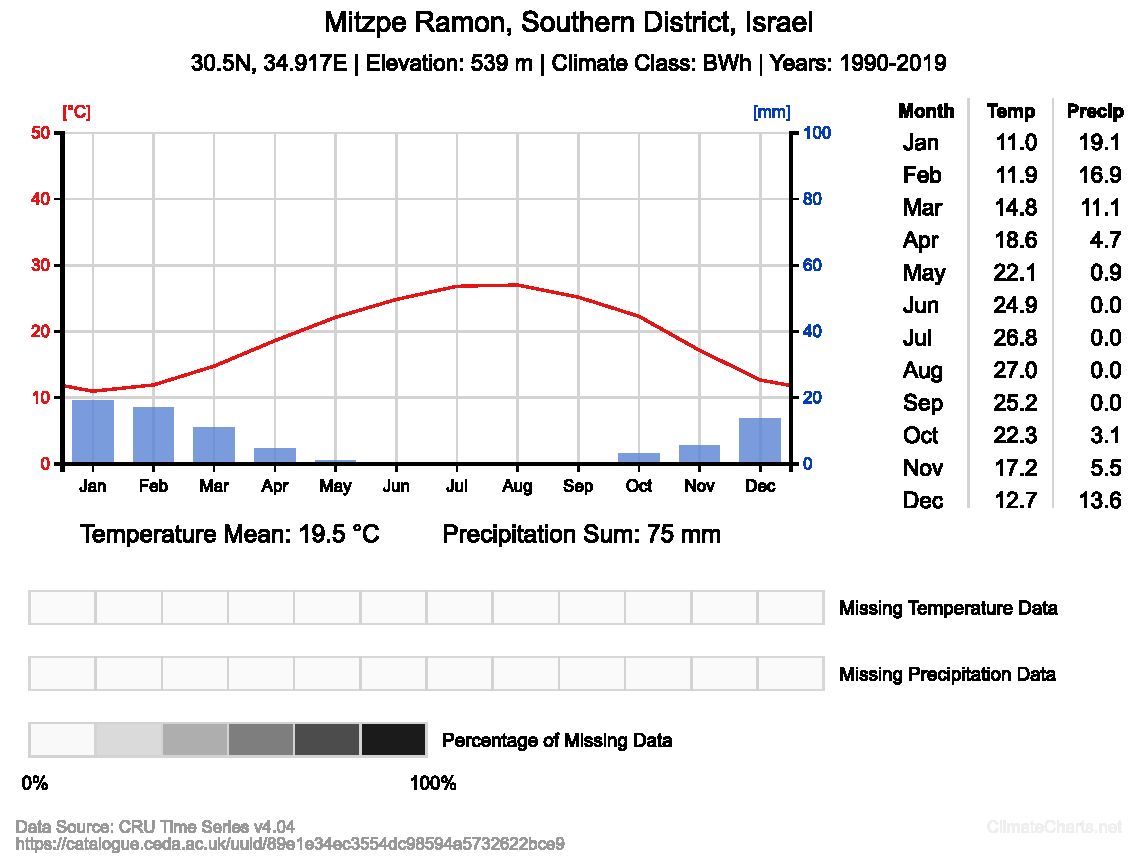
\includegraphics[width = 0.96\textwidth]{temp_maps/temp_negev}
  	\caption{Monthly averages of temperature and precipitation data for Mitzpe Ramon, Southern District, Israel (Negev Desert). (Image credit: \cite{Zepner:2020})}
	\label{fig:temp_negev}
\end{figure}

\begin{lstfloat}
\begin{lstlisting}[numbers = none, caption = {Output of the \MATLAB simulation in appendix \ref{sec:matlab_code} regarding the installation of the PV generator for the mission inputs in the table \ref{tab:table_negev}.}, label = lst:list_negev_1, captionpos = b]
              *******************************************
              [OUTPUT] PV GENERATOR INSTALLATION:

              Mission day | Opt. tilt angle | Orientation
              -------------------------------------------
              04-Oct-2021 |    35.78 deg    |    SOUTH
              05-Oct-2021 |    36.18 deg    |    SOUTH
              06-Oct-2021 |    36.57 deg    |    SOUTH
              07-Oct-2021 |    36.96 deg    |    SOUTH
              08-Oct-2021 |    37.34 deg    |    SOUTH
              09-Oct-2021 |    37.73 deg    |    SOUTH
              10-Oct-2021 |    38.11 deg    |    SOUTH
              11-Oct-2021 |    38.49 deg    |    SOUTH
              12-Oct-2021 |    38.87 deg    |    SOUTH
              13-Oct-2021 |    39.25 deg    |    SOUTH
              14-Oct-2021 |    39.62 deg    |    SOUTH
              15-Oct-2021 |    39.99 deg    |    SOUTH
              16-Oct-2021 |    40.36 deg    |    SOUTH
              17-Oct-2021 |    40.72 deg    |    SOUTH
              18-Oct-2021 |    41.08 deg    |    SOUTH
              19-Oct-2021 |    41.44 deg    |    SOUTH
              20-Oct-2021 |    41.80 deg    |    SOUTH
              21-Oct-2021 |    42.15 deg    |    SOUTH
              22-Oct-2021 |    42.50 deg    |    SOUTH
              23-Oct-2021 |    42.84 deg    |    SOUTH
              24-Oct-2021 |    43.18 deg    |    SOUTH
              25-Oct-2021 |    43.52 deg    |    SOUTH
              26-Oct-2021 |    43.86 deg    |    SOUTH
              27-Oct-2021 |    44.19 deg    |    SOUTH
              28-Oct-2021 |    44.51 deg    |    SOUTH
              29-Oct-2021 |    44.83 deg    |    SOUTH
              30-Oct-2021 |    45.15 deg    |    SOUTH
              31-Oct-2021 |    45.46 deg    |    SOUTH
              -------------------------------------------
                  Mean    |    40.80 deg    |    SOUTH

              *******************************************
\end{lstlisting}
\end{lstfloat}
Listing \ref{lst:list_negev_1} shows the optimal angle of inclination -- or tilting angle -- $\beta$ and the orientation of the normal to the PV generator's energy converting surface $A_\mathrm{PV}$, with respect to the cardinal directions, for each mission day. As explained in the subsection \ref{sec:photovoltaic_generator_alignment}, the optimal angle of inclination applies for solar noon $t_\mathrm{S} = 12\mathrm{h}$. This might not be true for cloudy days when the direct normal irradiation is weaker. During these days, $\beta$ must be reduced in order to maximize $E_\mathrm{DIFG}$ and $E_\mathrm{RGI}$ (copmare to equations \ref{eq:e_difg} and \ref{eq:e_rgi}), which causes $E_\mathrm{G}$ to increse (compare to equation \ref{eq:e_gen_ghi_dni}). Furthermore, the simulation determines the mean angle of inclination and orientation so that the PV generator only needs to be set up once at the beginning of the mission.

\begin{lstfloat}
\begin{lstlisting}[keywordstyle=\color{black}, numbers = none, caption = {Output of the \MATLAB simulation in appendix \ref{sec:matlab_code} regarding the daily energy yield of the PV generator for the mission inputs in the table \ref{tab:table_negev}.}, label = lst:list_negev_2, captionpos = b]
                 *************************************
                 [OUTPUT] PV GENERATOR ENERGY YIELD:

                 Applies for mean tilting angle and
                 orientation. The energy yield is 
                 the electrical energy yield. SOC 
                 full shows if the battery could be 
                 fully charged during the day.

                 Mission day | Energy yield | SOC full
                 -------------------------------------
                 04-Oct-2021 |   427.74 Wh  |    NO   
                 05-Oct-2021 |   428.65 Wh  |    NO   
                 06-Oct-2021 |   430.23 Wh  |    NO   
                 07-Oct-2021 |   431.09 Wh  |    NO   
                 08-Oct-2021 |   431.92 Wh  |    NO   
                 09-Oct-2021 |   433.41 Wh  |    NO   
                 10-Oct-2021 |   434.17 Wh  |   YES   
                 11-Oct-2021 |   435.61 Wh  |   YES   
                 12-Oct-2021 |   436.31 Wh  |   YES   
                 13-Oct-2021 |   437.69 Wh  |   YES   
                 14-Oct-2021 |   438.32 Wh  |   YES   
                 15-Oct-2021 |   439.64 Wh  |   YES   
                 16-Oct-2021 |   440.21 Wh  |   YES   
                 17-Oct-2021 |   441.46 Wh  |   YES   
                 18-Oct-2021 |   441.96 Wh  |   YES   
                 19-Oct-2021 |   443.15 Wh  |   YES   
                 20-Oct-2021 |   443.58 Wh  |   YES   
                 21-Oct-2021 |   444.71 Wh  |   YES   
                 22-Oct-2021 |   445.80 Wh  |   YES   
                 23-Oct-2021 |   446.12 Wh  |   YES   
                 24-Oct-2021 |   447.15 Wh  |   YES   
                 25-Oct-2021 |   447.40 Wh  |   YES   
                 26-Oct-2021 |   448.37 Wh  |   YES   
                 27-Oct-2021 |   449.30 Wh  |   YES   
                 28-Oct-2021 |   449.44 Wh  |   YES   
                 29-Oct-2021 |   450.30 Wh  |   YES   
                 30-Oct-2021 |   450.37 Wh  |   YES   
                 31-Oct-2021 |   451.16 Wh  |   YES   

                 *************************************
\end{lstlisting}
\end{lstfloat}
To display the command window output shown in the listing \ref{lst:list_negev_2}, the simulation uses the mean inclination angle from the listing \ref{lst:list_negev_1} and calculates the daily electrical energy yield of the PV generator. On the basis of this, the SOC of the battery is calculated for each mission day. An algorithm then evaluates whether the battery has been fully charged during each mission day and outputs either \codeword{YES} or \codeword{NO}. As it can be seen, the battery cannot be fully charged for the first few mission days. This is due to the assumption that the battery is $60\%$ charged at the beginning of the mission -- hence $\mathrm{SOC_{init}} = 0,6$. With this SOC, the Offgridtec Smart-Pro $12,8\mathrm{V}$ $50\mathrm{Ah}$ $\mathrm{LiFePO}_4$ battery is stored for longer periods of time \cite{Offgridtec:2020}. Therefore it can be said that the self-sufficient energy distribution system can supply the repeater radio system during the course of the analog Mars field mission AMADEE-20.

An interesting case occurs when the battery cannot be fully charged towards the end of the mission. This can happen, for instance, when the available solar energy is decreasing every day. Such results can be explained by changing seasons. In this case PV generators must be connected in parallel to guarantee sufficient electrical energy supply of the repeater radio system throughout the mission.

\begin{lstfloat}
\begin{lstlisting}[numbers = none, caption = {Output of the \MATLAB simulation in appendix \ref{sec:matlab_code} regarding the installation of the PV generator for the mission inputs in the table \ref{tab:table_vienna}.}, label = lst:list_negev_3, captionpos = b]
              *******************************************
              [OUTPUT] PV GENERATOR INSTALLATION:

              Mission day | Opt. tilt angle | Orientation
              -------------------------------------------
              01-Apr-2021 |    43.84 deg    |    SOUTH
              02-Apr-2021 |    43.44 deg    |    SOUTH
              03-Apr-2021 |    43.05 deg    |    SOUTH
              04-Apr-2021 |    42.65 deg    |    SOUTH
              05-Apr-2021 |    42.26 deg    |    SOUTH
              06-Apr-2021 |    41.87 deg    |    SOUTH
              07-Apr-2021 |    41.48 deg    |    SOUTH
              08-Apr-2021 |    41.10 deg    |    SOUTH
              09-Apr-2021 |    40.71 deg    |    SOUTH
              10-Apr-2021 |    40.33 deg    |    SOUTH
              11-Apr-2021 |    39.95 deg    |    SOUTH
              12-Apr-2021 |    39.58 deg    |    SOUTH
              13-Apr-2021 |    39.20 deg    |    SOUTH
              14-Apr-2021 |    38.83 deg    |    SOUTH
              15-Apr-2021 |    38.46 deg    |    SOUTH
              16-Apr-2021 |    38.10 deg    |    SOUTH
              17-Apr-2021 |    37.74 deg    |    SOUTH
              18-Apr-2021 |    37.38 deg    |    SOUTH
              19-Apr-2021 |    37.02 deg    |    SOUTH
              20-Apr-2021 |    36.67 deg    |    SOUTH
              21-Apr-2021 |    36.32 deg    |    SOUTH
              22-Apr-2021 |    35.97 deg    |    SOUTH
              23-Apr-2021 |    35.63 deg    |    SOUTH
              24-Apr-2021 |    35.29 deg    |    SOUTH
              25-Apr-2021 |    34.95 deg    |    SOUTH
              26-Apr-2021 |    34.62 deg    |    SOUTH
              27-Apr-2021 |    34.30 deg    |    SOUTH
              28-Apr-2021 |    33.97 deg    |    SOUTH
              29-Apr-2021 |    33.65 deg    |    SOUTH
              30-Apr-2021 |    33.34 deg    |    SOUTH
              -------------------------------------------
                  Mean    |    38.39 deg    |    SOUTH

              *******************************************
\end{lstlisting}
\end{lstfloat}
\begin{lstfloat}
\begin{lstlisting}[keywordstyle=\color{black}, numbers = none, caption = {Output of the \MATLAB simulation in appendix \ref{sec:matlab_code} regarding the daily energy yield of the PV generator for the mission inputs in the table \ref{tab:table_vienna}.}, label = lst:list_negev_4, captionpos = b]
                 *************************************
                 [OUTPUT] PV GENERATOR ENERGY YIELD:

                 Applies for mean tilting angle and
                 orientation. The energy yield is 
                 the electrical energy yield. SOC
                 full shows if the battery could be
                 fully charged during the day.

                 Mission day | Energy yield | SOC full
                 -------------------------------------
                 01-Apr-2021 |   490.62 Wh  |    NO   
                 02-Apr-2021 |   490.80 Wh  |    NO   
                 03-Apr-2021 |   490.98 Wh  |   YES   
                 04-Apr-2021 |   491.15 Wh  |   YES   
                 05-Apr-2021 |   491.31 Wh  |   YES   
                 06-Apr-2021 |   491.47 Wh  |   YES   
                 07-Apr-2021 |   491.62 Wh  |   YES   
                 08-Apr-2021 |   491.78 Wh  |   YES   
                 09-Apr-2021 |   491.93 Wh  |   YES   
                 10-Apr-2021 |   492.08 Wh  |   YES   
                 11-Apr-2021 |   492.23 Wh  |   YES   
                 12-Apr-2021 |   492.38 Wh  |   YES   
                 13-Apr-2021 |   492.53 Wh  |   YES   
                 14-Apr-2021 |   491.98 Wh  |   YES   
                 15-Apr-2021 |   492.16 Wh  |   YES   
                 16-Apr-2021 |   492.32 Wh  |   YES   
                 17-Apr-2021 |   492.48 Wh  |   YES   
                 18-Apr-2021 |   492.65 Wh  |   YES   
                 19-Apr-2021 |   492.83 Wh  |   YES   
                 20-Apr-2021 |   493.01 Wh  |   YES   
                 21-Apr-2021 |   492.51 Wh  |   YES   
                 22-Apr-2021 |   492.73 Wh  |   YES   
                 23-Apr-2021 |   492.94 Wh  |   YES   
                 24-Apr-2021 |   493.16 Wh  |   YES   
                 25-Apr-2021 |   492.70 Wh  |   YES   
                 26-Apr-2021 |   492.94 Wh  |   YES   
                 27-Apr-2021 |   493.23 Wh  |   YES   
                 28-Apr-2021 |   492.80 Wh  |   YES   
                 29-Apr-2021 |   493.09 Wh  |   YES   
                 30-Apr-2021 |   493.40 Wh  |   YES   

                 *************************************
\end{lstlisting}
\end{lstfloat}
A similar command window output can be obtained from the listings \ref{lst:list_negev_3} and \ref{lst:list_negev_4} for Vienna. Here, however, two PV generators connected in parallel are required. Besides that, simulations have shown, that the daily electrical energy yield is incresed when the angle of inlcination $\beta = 0^\circ$. This can also be recognized by analyzing the solar resources maps in the figures \ref{fig:ghi_austria} and \ref{fig:dni_austria}, because the global horizontal irradiation is greater than the direct normal irradiation. The author of the book \cite{Mertens:2015} mentions this as well. Such a simulation result can further be explained by the fact that these solar resource maps provide average values that have been recorded over several years and are therefore mainly used for the long-term planning of a PV generator array.

In order to obtain more intuitive simulation results, the SOC of the battery can be plotted over the entire duration of the mission or for individual mission days. Since the \MATLAB simulation only serves as a reference point, the on-site support crew still has to make regular checks of the battery's SOC during the mission in order to collect empirical data. Finally, it should be noted that the simulation could not provide any results for the DAS Energy DAS145PF PV generator, as it could not meet the condition $U_\mathrm{in,PV} > U_\mathrm{B} + 5\mathrm{V}$ with the solar resource maps mentioned. However, this could be different with the solar resource maps from \cite{Union:2020}. 

\begin{figure}[h!]
	\centering
  	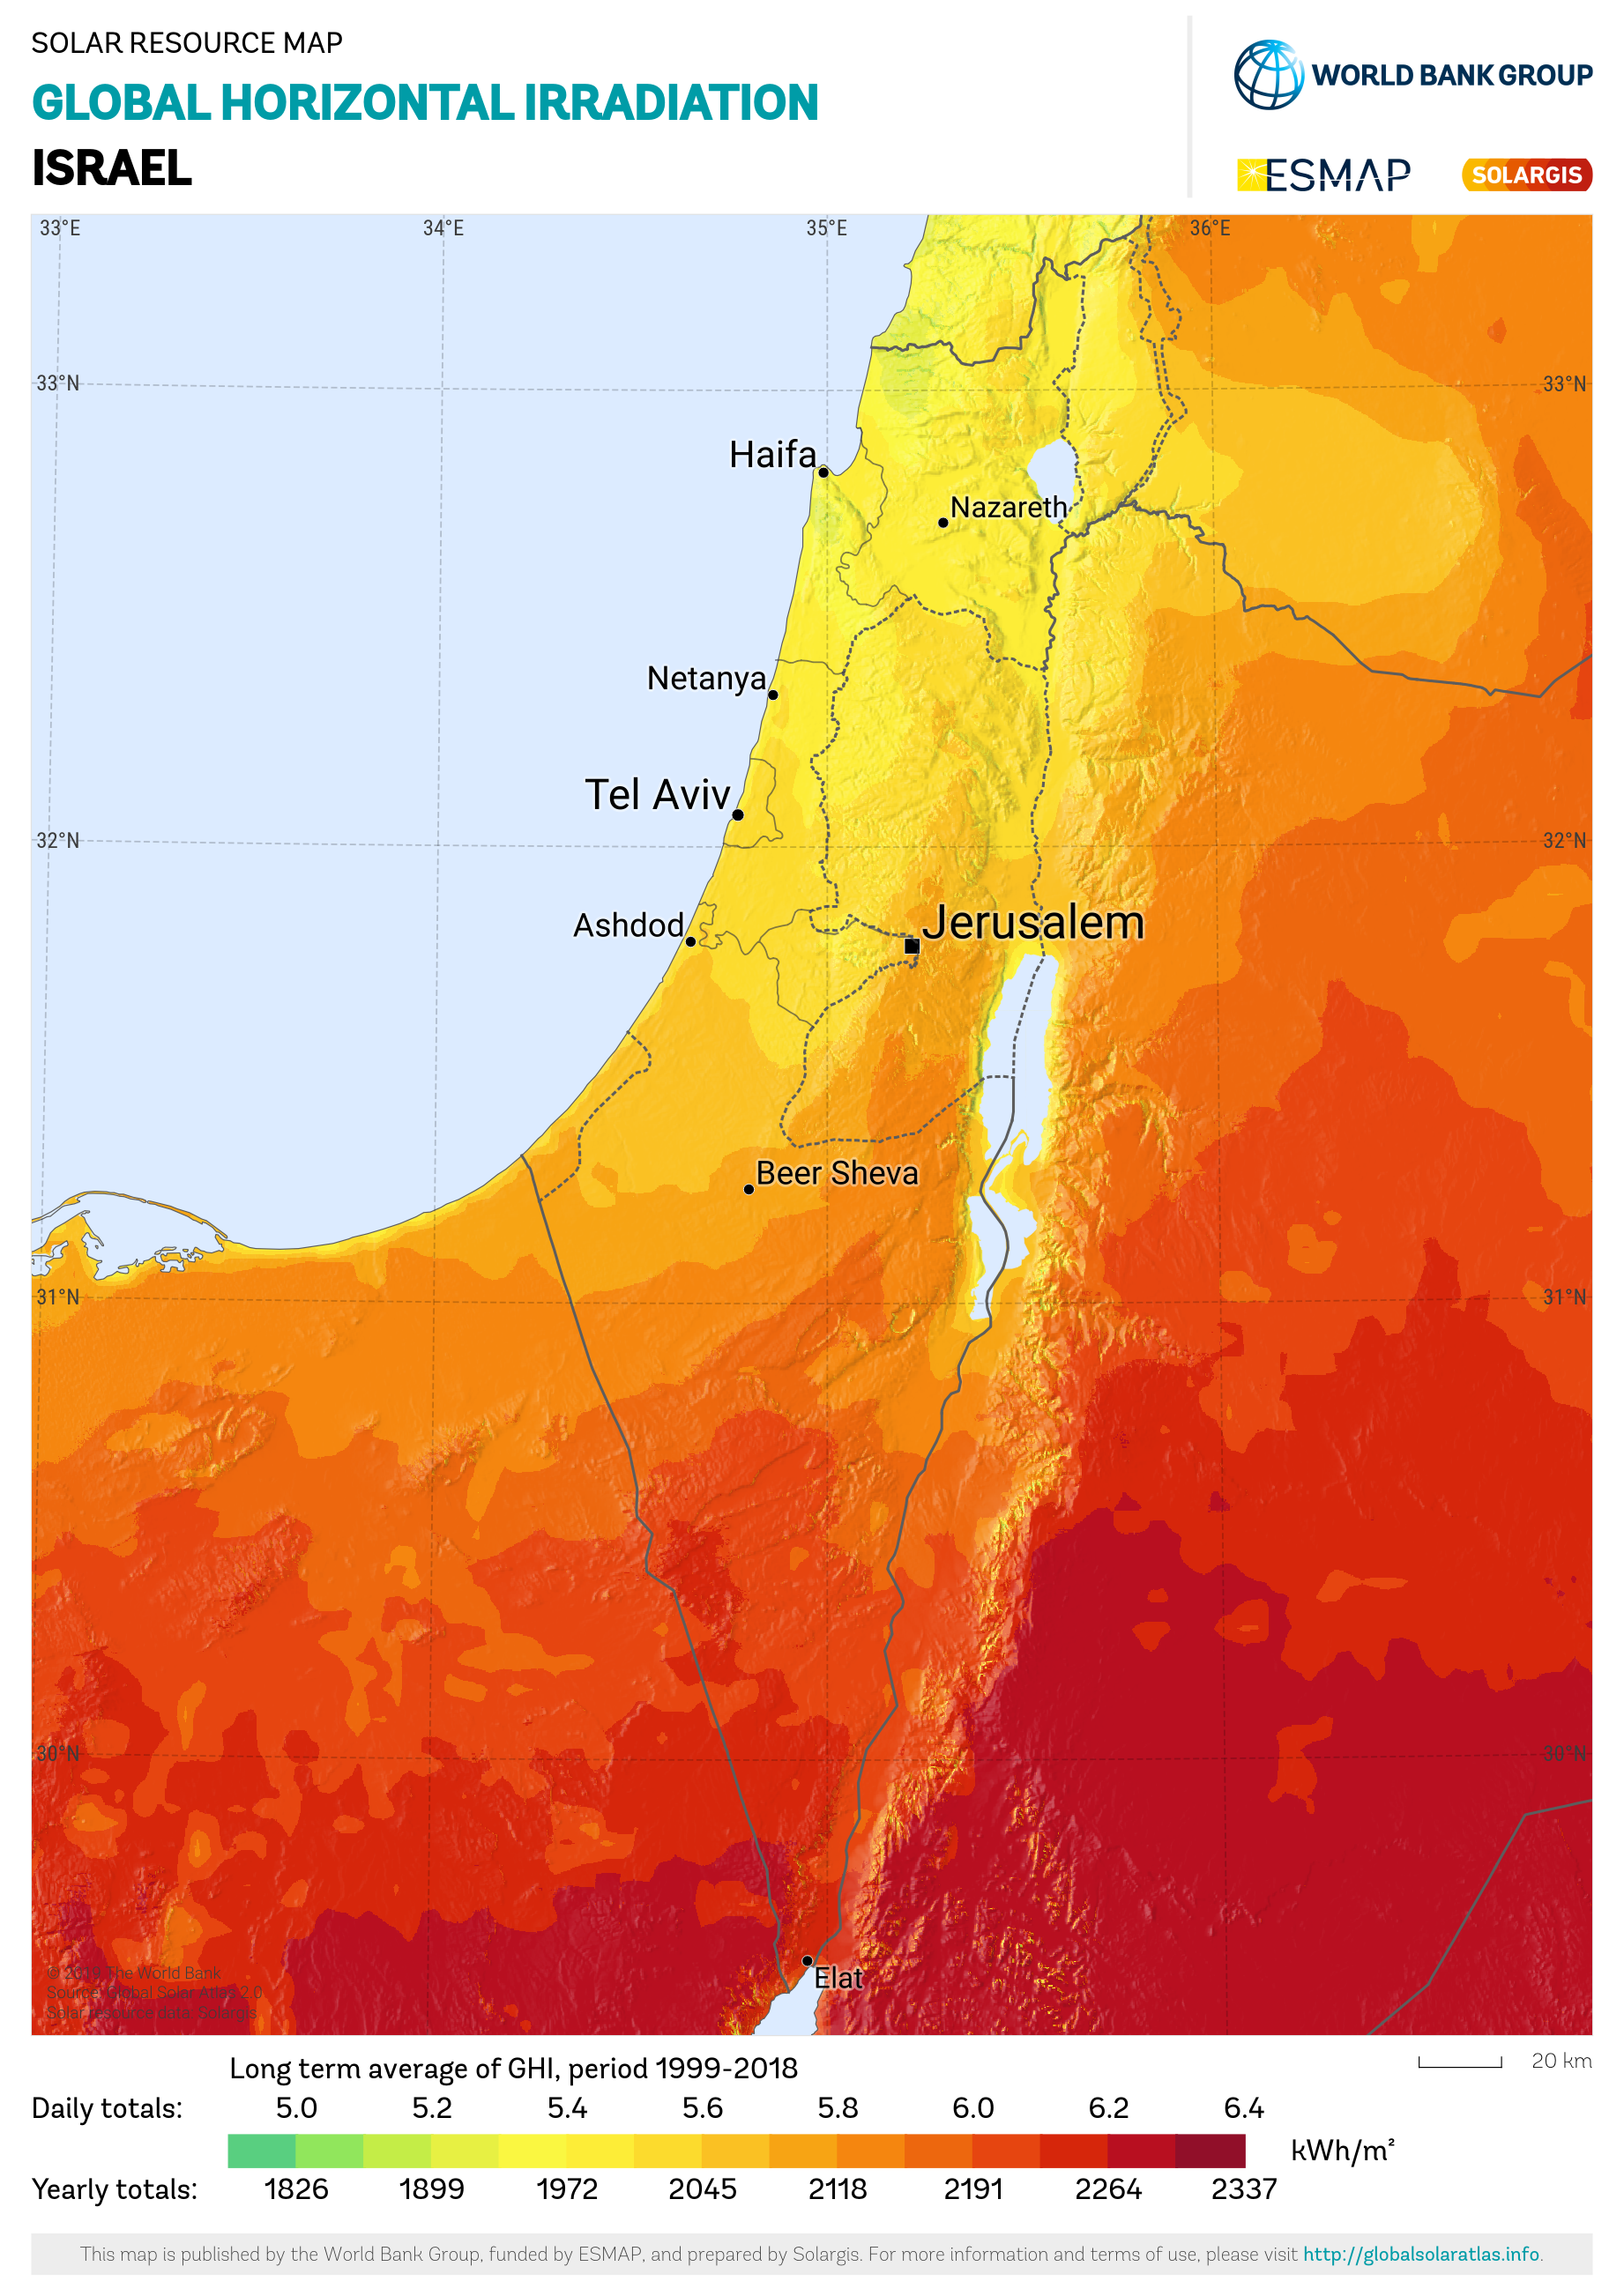
\includegraphics[width = \textwidth]{solar_maps/israel/israel_ghi}
  	\caption{Solar resource map of the long term average global horizontal irradiation of Israel. (Image credit: \cite{GlobalSolarAtlas:2020, Solargis:2021})}
	\label{fig:ghi_israel}
\end{figure}
\begin{figure}[h!]
	\centering
  	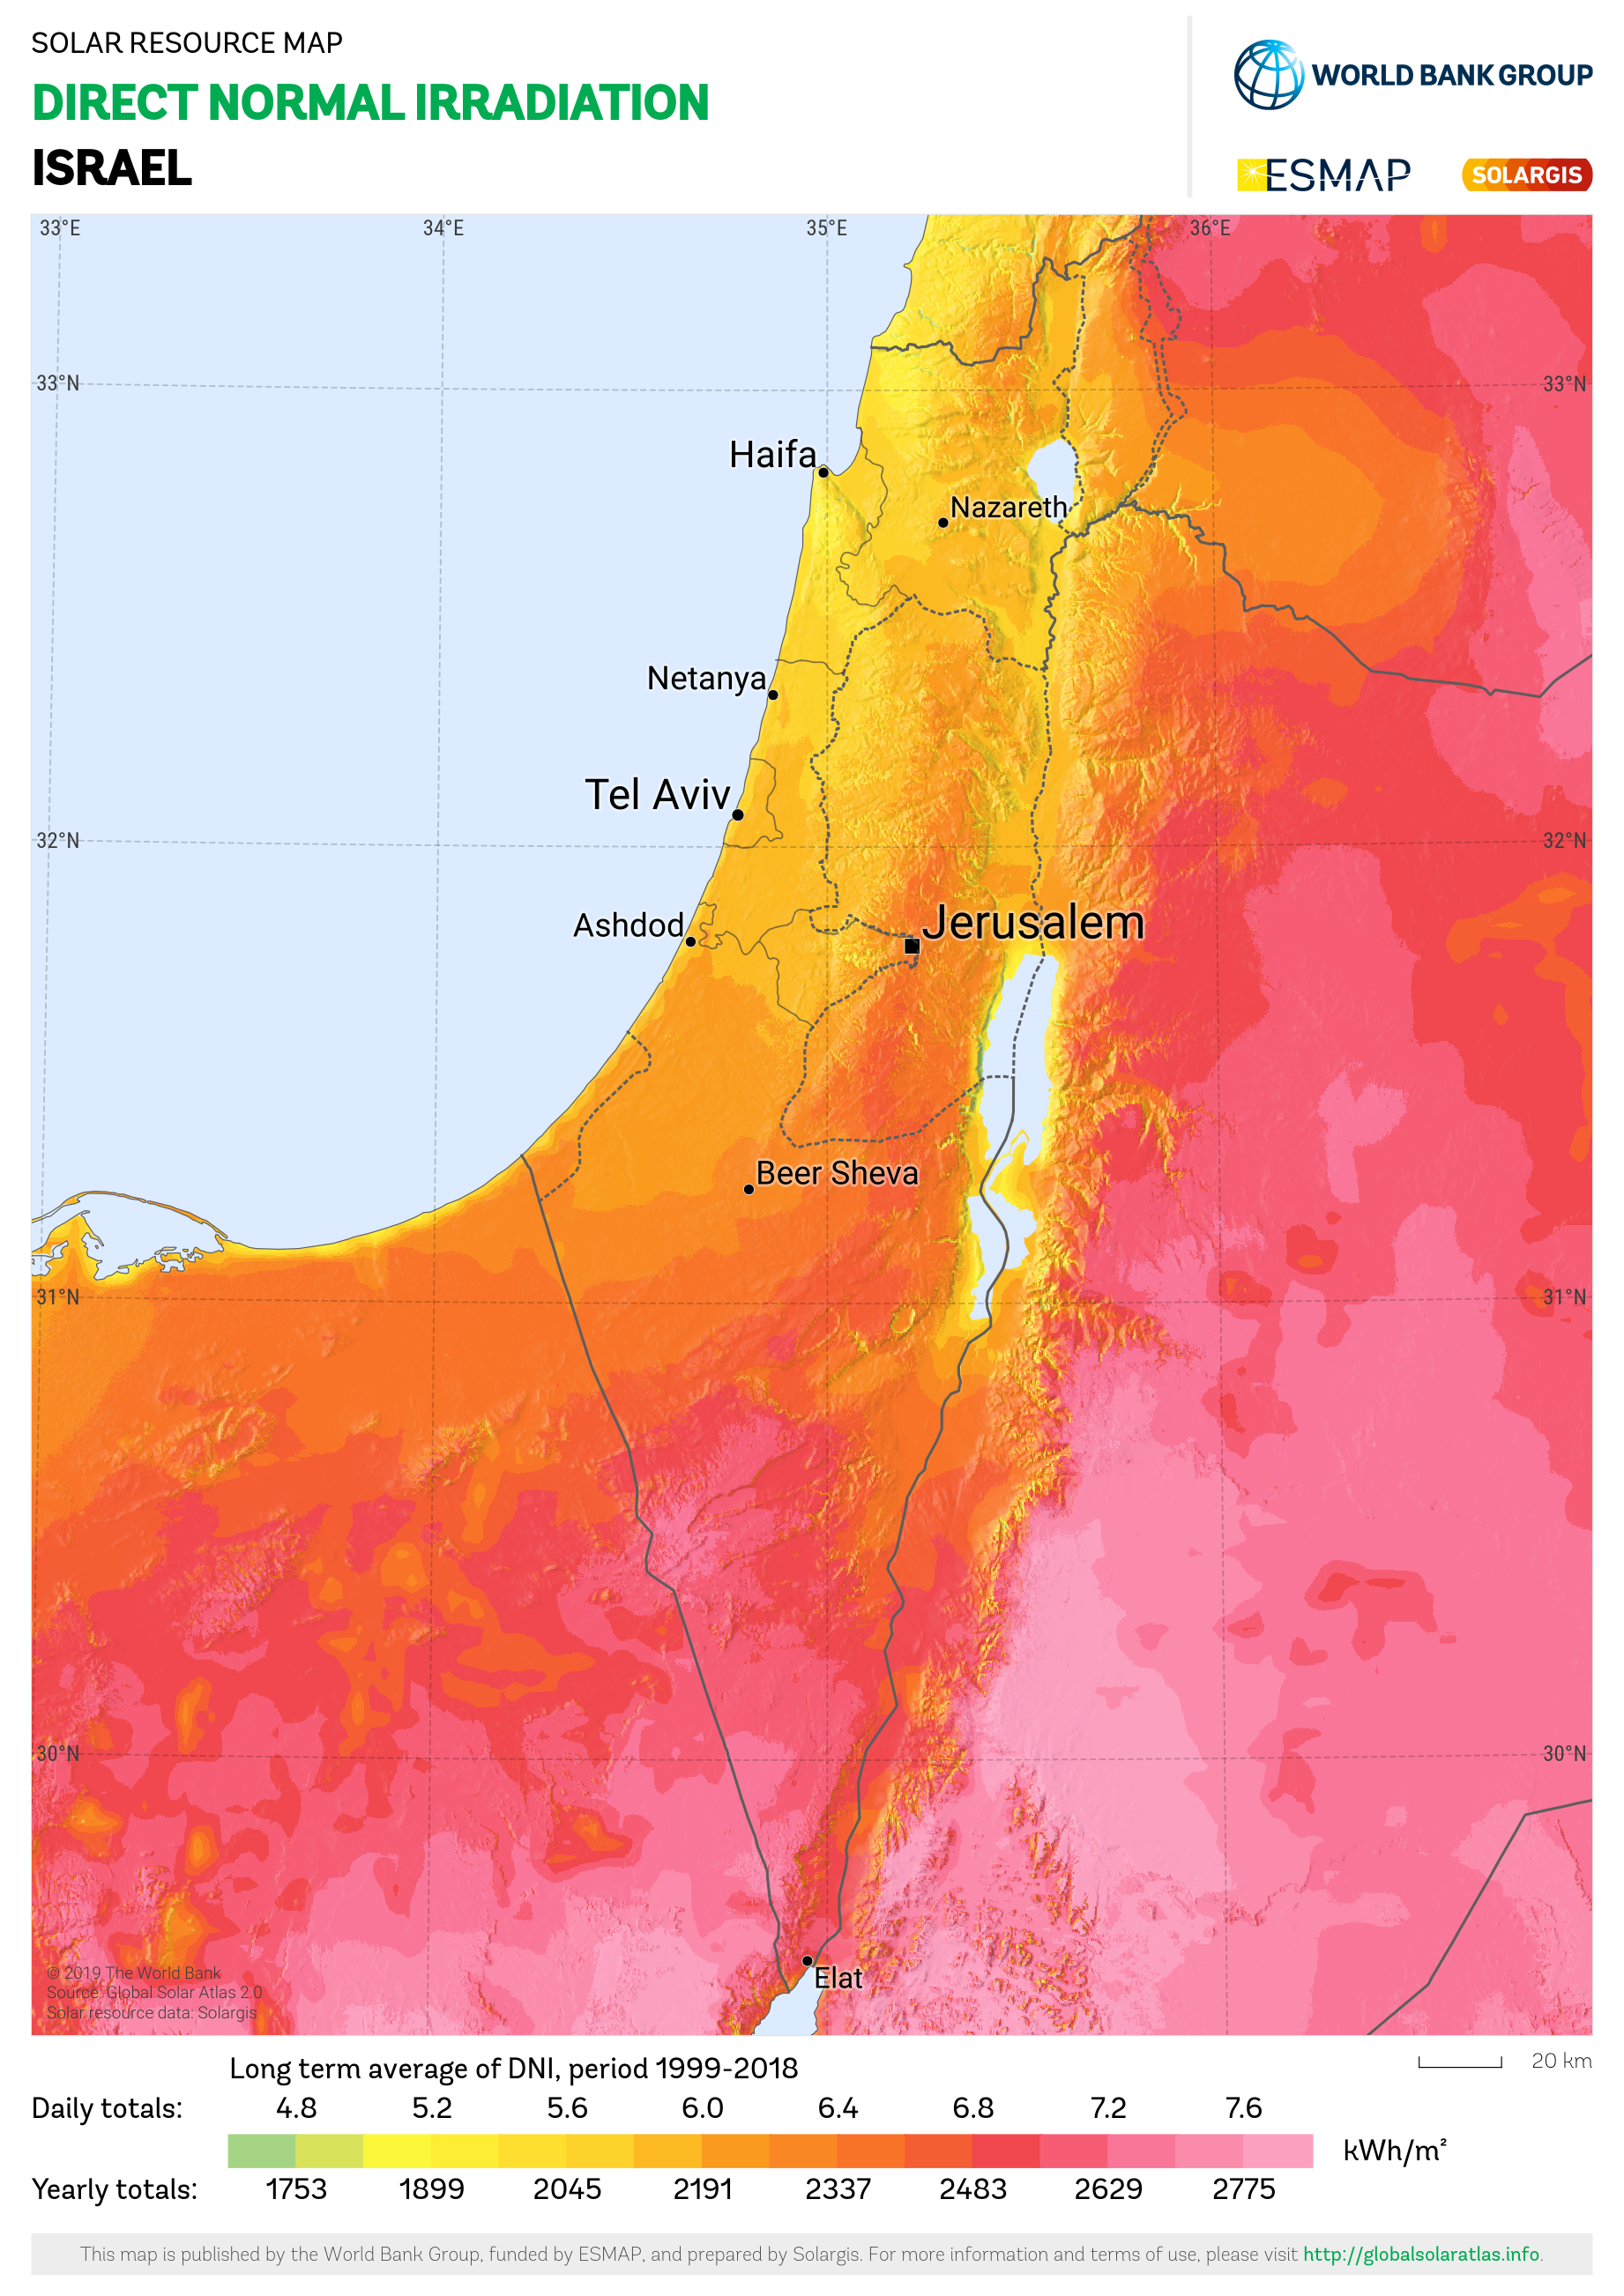
\includegraphics[width = \textwidth]{solar_maps/israel/israel_dni}
	\caption{Solar resource map of the long term average direct normal irradiation of Israel. (Image credit: \cite{GlobalSolarAtlas:2020, Solargis:2021})}
	\label{fig:dni_israel}
\end{figure}








% Warum wurde DAS Energy nicht verwendet!


% REFLECTION MAKE THE SIM BETTER AND MORE ACCURATE!!